% LuaLaTeX

\documentclass[a4paper, twoside, 12pt]{article}
\usepackage[latin]{babel}
%\usepackage[landscape, left=3cm, right=1.5cm, top=2cm, bottom=1cm]{geometry} % okraje stranky
\usepackage[portrait, a4paper, mag=1414, truedimen, left=0.8cm, right=0.8cm, top=0.8cm, bottom=0.8cm]{geometry} % okraje stranky

\usepackage{fontspec}
\setmainfont[FeatureFile={junicode.fea}, Ligatures={Common, TeX}, RawFeature=+fixi]{Junicode}
%\setmainfont{Junicode}

% shortcut for Junicode without ligatures (for the Czech texts)
\newfontfamily\nlfont[FeatureFile={junicode.fea}, Ligatures={Common, TeX}, RawFeature=+fixi]{Junicode}

\usepackage{multicol}
\usepackage{color}
\usepackage{lettrine}
\usepackage{fancyhdr}

% usual packages loading:
\usepackage{luatextra}
\usepackage{graphicx} % support the \includegraphics command and options
\usepackage{gregoriotex} % for gregorio score inclusion
\usepackage{gregoriosyms}
\usepackage{wrapfig} % figures wrapped by the text
\usepackage{parcolumns}
\usepackage[contents={},opacity=1,scale=1,color=black]{background}
\usepackage{tikzpagenodes}
\usepackage{calc}
\usepackage{longtable}

\setlength{\headheight}{12pt}

% Commands used to produce a typical "Conventus" booklet

\newenvironment{titulusOfficii}{\begin{center}}{\end{center}}
\newcommand{\dies}[1]{#1

}
\newcommand{\nomenFesti}[1]{\textbf{\Large #1}

}
\newcommand{\celebratio}[1]{#1

}

\newcommand{\hora}[1]{%
\vspace{0.5cm}{\large \textbf{#1}}

\fancyhead[LE]{\thepage\ / #1}
\fancyhead[RO]{#1 / \thepage}
\addcontentsline{toc}{subsection}{#1}
}

% larger unit than a hora
\newcommand{\divisio}[1]{%
\begin{center}
{\Large \textsc{#1}}
\end{center}
\fancyhead[CO,CE]{#1}
\addcontentsline{toc}{section}{#1}
}

% a part of a hora, larger than pars
\newcommand{\subhora}[1]{
\begin{center}
{\large \textit{#1}}
\end{center}
%\fancyhead[CO,CE]{#1}
\addcontentsline{toc}{subsubsection}{#1}
}

% rubricated inline text
\newcommand{\rubricatum}[1]{\textit{#1}}

% standalone rubric
\newcommand{\rubrica}[1]{\vspace{3mm}\rubricatum{#1}}

\newcommand{\notitia}[1]{\textcolor{red}{#1}}

\newcommand{\scriptura}[1]{\hfill \small\textit{#1}}

\newcommand{\translatioCantus}[1]{\vspace{1mm}%
{\noindent\footnotesize \nlfont{#1}}}

% pruznejsi varianta nasledujiciho - umoznuje nastavit sirku sloupce
% s prekladem
\newcommand{\psalmusEtTranslatioB}[3]{
  \vspace{0.5cm}
  \begin{parcolumns}[colwidths={2=#3}, nofirstindent=true]{2}
    \colchunk{
      \input{#1}
    }

    \colchunk{
      \vspace{-0.5cm}
      {\footnotesize \nlfont
        \input{#2}
      }
    }
  \end{parcolumns}
}

\newcommand{\psalmusEtTranslatio}[2]{
  \psalmusEtTranslatioB{#1}{#2}{8.5cm}
}


\newcommand{\canticumMagnificatEtTranslatio}[1]{
  \psalmusEtTranslatioB{#1}{temporalia/extra-adventum-vespers/magnificat-boh.tex}{12cm}
}
\newcommand{\canticumBenedictusEtTranslatio}[1]{
  \psalmusEtTranslatioB{#1}{temporalia/extra-adventum-laudes/benedictus-boh.tex}{10.5cm}
}

% volne misto nad antifonami, kam si zpevaci dokresli neumy
\newcommand{\hicSuntNeumae}{\vspace{0.5cm}}

% prepinani mista mezi notovymi osnovami: pro neumovane a neneumovane zpevy
\newcommand{\cantusCumNeumis}{
  \setgrefactor{17}
  \global\advance\grespaceabovelines by 5mm%
}
\newcommand{\cantusSineNeumas}{
  \setgrefactor{17}
  \global\advance\grespaceabovelines by -5mm%
}

% znaky k umisteni nad inicialu zpevu
\newcommand{\superInitialam}[1]{\gresetfirstlineaboveinitial{\small {\textbf{#1}}}{\small {\textbf{#1}}}}

% pars officii, i.e. "oratio", ...
\newcommand{\pars}[1]{\textbf{#1}}

\newenvironment{psalmus}{
  \setlength{\parindent}{0pt}
  \setlength{\parskip}{5pt}
}{
  \setlength{\parindent}{10pt}
  \setlength{\parskip}{10pt}
}

%%%% Prejmenovat na latinske:
\newcommand{\nadpisZalmu}[1]{
  \hspace{2cm}\textbf{#1}\vspace{2mm}%
  \nopagebreak%

}

% mode, score, translation
\newcommand{\antiphona}[3]{%
\hicSuntNeumae
\superInitialam{#1}
\includescore{#2}

#3
}
 % Often used macros

\setlength{\columnsep}{15pt} % prostor mezi sloupci

%%%%%%%%%%%%%%%%%%%%%%%%%%%%%%%%%%%%%%%%%%%%%%%%%%%%%%%%%%%%%%%%%%%%%%%%%%%%%%%%%%%%%%%%%%%%%%%%%%%%%%%%%%%%%
\begin{document}

% Here we set the space around the initial.
% Please report to http://home.gna.org/gregorio/gregoriotex/details for more details and options
\grechangedim{afterinitialshift}{2.2mm}{scalable}
\grechangedim{beforeinitialshift}{2.2mm}{scalable}
\grechangedim{interwordspacetext}{0.38 cm plus 0.15 cm minus 0.05 cm}{scalable}%
\grechangedim{annotationraise}{-0.2cm}{scalable}

% Here we set the initial font. Change 38 if you want a bigger initial.
% Emit the initials in red.
\grechangestyle{initial}{\color{red}\fontsize{36}{36}\selectfont}

\renewcommand{\headrulewidth}{0pt} % no horiz. rule at the header
\pagestyle{empty}

\grechangedim{spaceabovelines}{0.2cm}{scalable}%

\vfill

\hbox{}

\vspace{5cm}

\begin{center}
{\large \textit{DIE XX IULII}}

\vspace{0.5cm}

{\huge S. MARGARITÆ}

{\large VIRGINIS ET MARTYRIS}

\vspace{0.5cm}

% graphic
\vspace{1.5cm}
\begin{center}
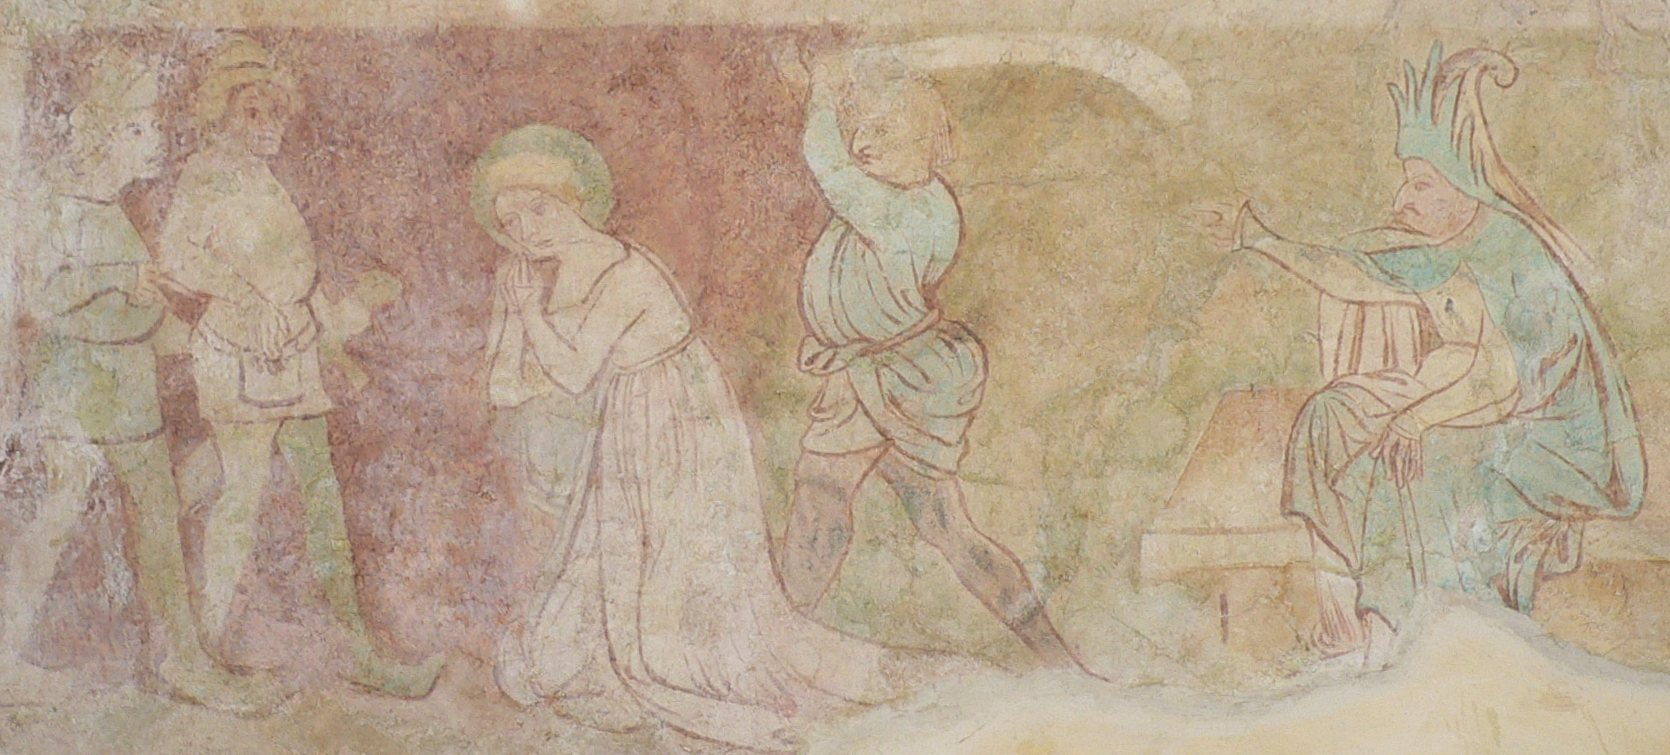
\includegraphics[width=8cm]{margarita.jpg}
\end{center}

\vspace{0.5cm}

%\textsc{Secundum Antiphonale Breunowiensis}
\textsc{Secundum Antiphonale Raygradensis}
\end{center}

\vfill
\pagebreak

\cantusSineNeumas

\pars{Introductio}

\gregorioscore{temporalia/deusinadiutorium-communis.gtex}

\vspace{0.5cm}

\pars{Antiphona I}

\vspace{-0.2cm}

\antiphona{II D}{temporalia/ant1.gtex}

\scriptura{Ps. 109}

\gregorioscore{temporalia/ps109-initium-ii-D-auto.gtex}

{\setlength{\parindent}{0pt}\input{temporalia/ps109.tex}}

\vfill
\pagebreak

\pars{Antiphona II}

\vspace{-0.2cm}

\antiphona{III g}{temporalia/ant2.gtex}

\scriptura{Ps. 110}

%\grechangedim{interwordspacetext}{0.25 cm plus 0.15 cm minus 0.05 cm}{scalable}%
\gregorioscore{temporalia/ps110-initium-iii-g-auto.gtex}
%\grechangedim{interwordspacetext}{0.38 cm plus 0.15 cm minus 0.05 cm}{scalable}%

{\setlength{\parindent}{0pt}\input{temporalia/ps110.tex}}

\vfill
\pagebreak

\pars{Antiphona III}

\vspace{-0.2cm}

\antiphona{IV E}{temporalia/ant3.gtex}

\scriptura{Ps. 111}

%\grechangedim{interwordspacetext}{0.25 cm plus 0.15 cm minus 0.05 cm}{scalable}%
\gregorioscore{temporalia/ps111-initium-iv-E-auto.gtex}
%\grechangedim{interwordspacetext}{0.38 cm plus 0.15 cm minus 0.05 cm}{scalable}%

{\setlength{\parindent}{0pt}\input{temporalia/ps111.tex}}

\vfill
\pagebreak

\pars{Antiphona IV}

\vspace{-0.2cm}

\antiphona{V a}{temporalia/ant4.gtex}

\scriptura{Ps. 112}

%\grechangedim{interwordspacetext}{0.25 cm plus 0.15 cm minus 0.05 cm}{scalable}%
\gregorioscore{temporalia/ps112-initium-v-a-auto.gtex}
%\grechangedim{interwordspacetext}{0.38 cm plus 0.15 cm minus 0.05 cm}{scalable}%

{\setlength{\parindent}{0pt}\input{temporalia/ps112.tex}}

\vfill
\pagebreak

\pars{Antiphona V}

\vspace{-0.2cm}

\antiphona{VI C}{temporalia/ant5.gtex}

\scriptura{Ps. 113}

%\grechangedim{interwordspacetext}{0.25 cm plus 0.15 cm minus 0.05 cm}{scalable}%
\gregorioscore{temporalia/ps113-initium-vi-C-auto.gtex}
%\grechangedim{interwordspacetext}{0.38 cm plus 0.15 cm minus 0.05 cm}{scalable}%

{\setlength{\parindent}{0pt}\input{temporalia/ps113.tex}}

\vfill
\pagebreak

\pars{Capitulum} \scriptura{2 Cor. 10, 17-18}

Fratres: Qui gloriátur, in Dómino gloriétur.~\gredagger{}
Non enim qui seípsum comméndat, ille probátus est:~\grestar{}
sed quem Deus comméndat.

\vspace{0.5cm}

\pars{Responsorium breve}

\vspace{-0.2cm}

\antiphona{\oldrbar.~ br.}{temporalia/resp.gtex}

\vfill
\pagebreak

\pars{Hymnus}

\vspace{-0.5cm}

\antiphona{I}{temporalia/hym-VirginisProles.gtex}

\vspace{0.5cm}

\Vbardot{} Diffúsa est grátia in lábiis tuis.
\Rbardot{} Proptérea benedíxit te Deus in ætérnum.

\vfill
\pagebreak

\pars{Antiphona ad Magnificat}

\vspace{-0.2cm}

\antiphona{I g}{temporalia/ant-magn-vesp.gtex}

\scriptura{Lc. 1, 46-55}

\gregorioscore{temporalia/magnificat-initium-i-g.gtex}

{\setlength{\parindent}{0pt}\input{temporalia/magnificat.tex}}

\vfill
\pagebreak

\vspace{0.5cm}

\pars{Oratio conclusiva}

\gregorioscore{temporalia/oratio.gtex}

\end{document}
